\documentclass[11pt,aspectratio=169]{beamer}

\usepackage{booktabs}
\usepackage{array}
\usepackage{tikz}
\usepackage{pgfplots}
\usepackage{xcolor}
\usepackage{amsmath}
\usepackage{mathtools}
\usepackage{listings}
\usetikzlibrary{positioning,calc,arrows.meta,decorations.pathreplacing}
\pgfplotsset{compat=1.18}

\usetheme[titleformat=smallcaps,progressbar=frametitle]{metropolis}
\definecolor{UTburnt}{HTML}{BF5700}
\definecolor{LBJnavy}{HTML}{172A46}
\definecolor{softgray}{HTML}{F2F3F5}
\definecolor{midgray}{HTML}{6B7280}
\definecolor{softorange}{HTML}{F9E7DA}
\setbeamercolor{alerted text}{fg=UTburnt}
\setbeamercolor{frametitle}{bg=LBJnavy,fg=white}
\setbeamercolor{progress bar}{fg=UTburnt,bg=gray!25}
\setbeamercolor{block title}{bg=LBJnavy!10,fg=LBJnavy}
\setbeamercolor{block body}{bg=softgray}
\setbeamertemplate{navigation symbols}{}
\setbeamertemplate{itemize item}{\color{UTburnt}$\blacktriangleright$}
\setbeamertemplate{itemize subitem}{\color{UTburnt}$\bullet$}

\lstset{
  basicstyle=\ttfamily\scriptsize,
  backgroundcolor=\color{softgray},
  frame=single,
  rulecolor=\color{midgray!40},
  columns=fullflexible,
  keepspaces=true,
  showstringspaces=false
}

\author{Sergio I. Garc\'ia-R\'ios}
\title{Sampling Variability and the Central Limit Theorem}
\subtitle{Why samples differ, and why averages become predictable}
\institute{PA 311N: Data Analysis for Public Policy\\LBJ School of Public Affairs}
\date{October 5, 2026}

\newcommand{\yourturn}[1]{%
\begin{center}
\begin{minipage}{0.90\textwidth}
\begin{alertblock}{Your Turn}
#1
\end{alertblock}
\end{minipage}
\end{center}}

\newcommand{\ourturn}[1]{%
\begin{center}
\begin{minipage}{0.90\textwidth}
\begin{block}{Our Turn}
#1
\end{block}
\end{minipage}
\end{center}}

\newcommand{\SE}{\operatorname{SE}}

\begin{document}

\begin{frame}[plain]
\centering
\vspace{0.6cm}
{\color{LBJnavy}\LARGE\bfseries Sampling Variability and the Central Limit Theorem\par}
\vspace{0.4cm}
{\large Why samples differ, and why averages become predictable\par}
\vspace{0.9cm}
{\normalsize Sergio I. Garc\'ia-R\'ios\par}
\vspace{0.2cm}
{\small PA 311N: Data Analysis for Public Policy\par}
{\small LBJ School of Public Affairs\par}
\vfill
{\small October 5, 2026\par}
\end{frame}

% 2
\begin{frame}{Where we are going}
Last week we asked how probability models describe \alert{individual observations}.

\vspace{0.7em}
Today we ask a different question:

\begin{center}
\Large If we repeatedly draw samples,\\
\alert{how will our estimates vary?}
\end{center}

\vspace{0.7em}
That question is the bridge from descriptive statistics to statistical inference.
\end{frame}

% 3
\begin{frame}{The puzzle behind statistical inference}
Public policy rarely gives us the whole population.

\begin{itemize}
  \item We want a \alert{population parameter}: $\mu$, $p$, a difference, a regression coefficient.
  \item We observe a \alert{sample statistic}: $\bar{x}$, $\hat p$, and so on.
  \item A different random sample would usually give a different statistic.
\end{itemize}

\vspace{0.8em}
\begin{alertblock}{The puzzle}
If estimates change from sample to sample, why should we trust any one sample?
\end{alertblock}

\vfill
Today: because the variation itself has a pattern we can model.
\end{frame}

% 4
\begin{frame}{Population parameter vs. sample statistic}
\begin{columns}[T,onlytextwidth]
\column{0.47\textwidth}
\begin{block}{Population}
All 2,930 residential home sales in the Ames data.

\[
\mu = 1499.69\text{ sq. ft.}
\]

\[
\sigma = 505.51\text{ sq. ft.}
\]
\end{block}
\column{0.47\textwidth}
\begin{block}{One random sample}
Suppose we observe only $n=50$ homes.

\[
\bar{x}=\text{mean area in those 50 homes}
\]

The value of $\bar{x}$ depends on which homes were sampled.
\end{block}
\end{columns}

\vfill
\alert{$\mu$ is fixed. $\bar{x}$ varies.}
\end{frame}

% 5
\begin{frame}{One population, many possible samples}
Suppose two analysts independently draw 50 homes from the same population.

\begin{columns}[T,onlytextwidth]
\column{0.46\textwidth}
\begin{block}{Analyst A}
A random sample might produce
\[
\bar{x}=1417\text{ sq. ft.}
\]
\end{block}
\column{0.46\textwidth}
\begin{block}{Analyst B}
Another random sample might produce
\[
\bar{x}=1660\text{ sq. ft.}
\]
\end{block}
\end{columns}

\vspace{0.8em}
Both analysts used the same population and the same sample size.

\vfill
\alert{Different estimates are an expected consequence of random sampling.}
\end{frame}

% 6
\begin{frame}{Sampling variability is not automatically an error}
\begin{columns}[T,onlytextwidth]
\column{0.46\textwidth}
\begin{block}{Sampling variability}
Natural variation in a statistic because different random samples contain different observations.
\end{block}
\column{0.46\textwidth}
\begin{block}{Bias or bad measurement}
A systematic problem that pushes estimates in a particular direction.
\end{block}
\end{columns}

\vspace{0.8em}
A perfectly designed random sample still has sampling variability.

\vfill
\yourturn{If two high-quality polls of the same population report 47\% and 49\%, must one of them be wrong?}
\end{frame}

% 7
\begin{frame}[standout]
\Large We need a distribution\\of the statistic itself.
\end{frame}

% 8
\begin{frame}{Three different distributions}
\begin{enumerate}
  \item \textbf{Population distribution}: values for every unit in the population.
  \item \textbf{Sample distribution}: observed values in one particular sample.
  \item \textbf{Sampling distribution}: values of a statistic across many possible samples of the same size.
\end{enumerate}

\vspace{0.9em}
For the mean:
\[
\boxed{\text{sampling distribution of }\bar{x}}
\]

\vfill
The observations in a sampling distribution are \alert{sample means}, not individual homes or people.
\end{frame}

% 9
\begin{frame}{How a sampling distribution is constructed}
\centering
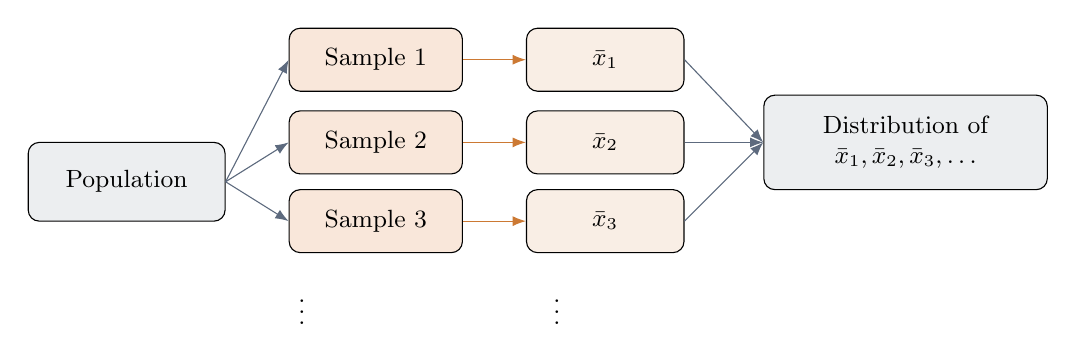
\begin{tikzpicture}[node distance=0.75cm and 0.8cm, every node/.style={font=\small}]
\node[draw,rounded corners,fill=LBJnavy!8,minimum width=2.5cm,minimum height=1cm] (pop) {Population};
\node[draw,rounded corners,fill=softorange,minimum width=2.2cm,minimum height=0.8cm,right=of pop,yshift=1.55cm] (s1) {Sample 1};
\node[draw,rounded corners,fill=softorange,minimum width=2.2cm,minimum height=0.8cm,right=of pop,yshift=0.5cm] (s2) {Sample 2};
\node[draw,rounded corners,fill=softorange,minimum width=2.2cm,minimum height=0.8cm,right=of pop,yshift=-0.5cm] (s3) {Sample 3};
\node[right=of pop,yshift=-1.55cm] (dots) {$\vdots$};
\node[draw,rounded corners,fill=UTburnt!10,minimum width=2.0cm,minimum height=0.8cm,right=of s1] (m1) {$\bar{x}_1$};
\node[draw,rounded corners,fill=UTburnt!10,minimum width=2.0cm,minimum height=0.8cm,right=of s2] (m2) {$\bar{x}_2$};
\node[draw,rounded corners,fill=UTburnt!10,minimum width=2.0cm,minimum height=0.8cm,right=of s3] (m3) {$\bar{x}_3$};
\node[right=of dots,xshift=2.1cm] (dots2) {$\vdots$};
\node[draw,rounded corners,fill=LBJnavy!8,minimum width=3.6cm,minimum height=1.2cm,right=1.0cm of m2,align=center] (dist) {Distribution of\\$\bar{x}_1,\bar{x}_2,\bar{x}_3,\ldots$};
\foreach \s in {s1,s2,s3}{\draw[-{Latex},LBJnavy!70] (pop.east) -- (\s.west);}
\draw[-{Latex},UTburnt!80] (s1.east)--(m1.west);
\draw[-{Latex},UTburnt!80] (s2.east)--(m2.west);
\draw[-{Latex},UTburnt!80] (s3.east)--(m3.west);
\draw[-{Latex},LBJnavy!70] (m1.east)--(dist.west);
\draw[-{Latex},LBJnavy!70] (m2.east)--(dist.west);
\draw[-{Latex},LBJnavy!70] (m3.east)--(dist.west);
\end{tikzpicture}

\vspace{0.7em}
\alert{Same population. Same $n$. New random sample each time.}
\end{frame}

% 10
\begin{frame}{Your turn: what does each dot represent?}
\yourturn{Imagine a histogram built from 5,000 values of $\bar{x}$, each calculated from a random sample of 50 Ames homes.

What does \textbf{one observation} in that histogram represent?}

\vspace{1em}
\begin{center}
\Large One \alert{sample mean} from one random sample of 50 homes.
\end{center}
\end{frame}

% 11
\begin{frame}{Ames gives us a useful experiment}
The population distribution of living area is \alert{right-skewed}:

\begin{center}
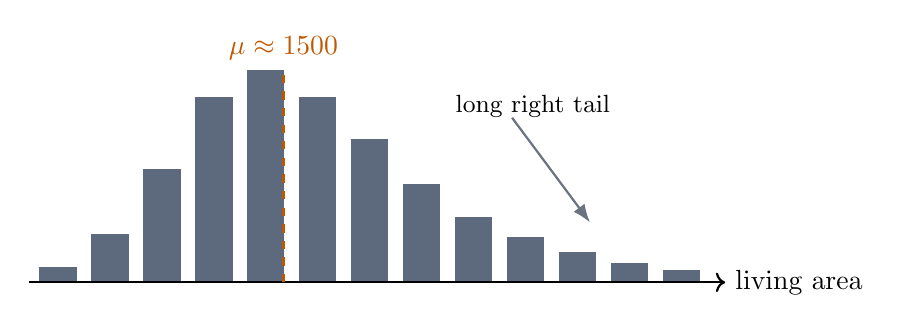
\begin{tikzpicture}[x=0.66cm,y=0.38cm]
\foreach \x/\h in {0/0.5,1/1.6,2/3.8,3/6.2,4/7.1,5/6.2,6/4.8,7/3.3,8/2.2,9/1.5,10/1.0,11/0.65,12/0.4}{
  \fill[LBJnavy!70] (\x,0) rectangle +(0.72,\h);
}
\draw[->,thick] (-0.2,0)--(13.2,0) node[right] {living area};
\draw[dashed,UTburnt,very thick] (4.7,0)--(4.7,7.1);
\node[above,UTburnt] at (4.7,7.1) {$\mu\approx1500$};
\node[align=center,font=\small] at (9.5,5.9) {long right tail};
\draw[-{Latex},midgray,thick] (9.1,5.5)--(10.6,2.0);
\end{tikzpicture}
\end{center}

\[
\mu=1499.69,\qquad \sigma=505.51.
\]

\vspace{0.15em}
This is useful because the raw population is \emph{not} perfectly normal.
\end{frame}

% 12
\begin{frame}{Standard deviation vs. standard error}
\begin{columns}[T,onlytextwidth]
\column{0.47\textwidth}
\begin{block}{Standard deviation, $\sigma$}
Describes variation among \alert{individual observations} in the population.

For Ames area:
\[
\sigma\approx505.5\text{ sq. ft.}
\]
\end{block}
\column{0.47\textwidth}
\begin{block}{Standard error, $\SE(\bar{x})$}
Describes variation among \alert{sample means} across repeated samples.

For $n=100$:
\[
\SE(\bar{x})\approx50.6\text{ sq. ft.}
\]
\end{block}
\end{columns}

\vfill
\alert{SD describes people/homes/units. SE describes estimates.}
\end{frame}

% 13
\begin{frame}{The standard error of the sample mean}
When observations are independent,

\[
\boxed{\SE(\bar{x})=\frac{\sigma}{\sqrt{n}}}
\]

\begin{itemize}
  \item More population variability ($\sigma$ larger) $\Rightarrow$ more uncertainty.
  \item Larger sample size ($n$ larger) $\Rightarrow$ less uncertainty.
  \item The benefit of sample size follows a \alert{square-root law}.
\end{itemize}

\vfill
In practice $\sigma$ is usually unknown; later we will estimate it using $s$.
\end{frame}

% 14
\begin{frame}{Sampling distribution for $n=10$}
For samples of 10 homes:
\[
\SE(\bar{x})=\frac{505.51}{\sqrt{10}}\approx160\text{ sq. ft.}
\]

\begin{center}
\begin{tikzpicture}
\begin{axis}[
  width=0.78\textwidth,height=0.42\textheight,
  xmin=850,xmax=2150,ymin=0,ymax=0.0029,
  axis lines=left,ytick=\empty,xtick={1000,1250,1500,1750,2000},
  xlabel={sample mean area, $\bar{x}$},
  tick label style={font=\small},label style={font=\small}
]
% Stylized: with a skewed population and small n, some skew can remain.
\addplot[LBJnavy,very thick,domain=850:2150,samples=180]
 {0.92*(1/(140*sqrt(2*pi))*exp(-((x-1472.6)^2)/(2*140^2)))
 +0.08*(1/(100*sqrt(2*pi))*exp(-((x-1815)^2)/(2*100^2)))};
\addplot[UTburnt,dashed,thick] coordinates {(1499.69,0) (1499.69,0.00275)};
\end{axis}
\end{tikzpicture}
\end{center}

\vspace{-0.4em}
The distribution is centered near the population mean, but with $n=10$ some skew may remain.
\end{frame}

% 15
\begin{frame}{Sampling distribution for $n=50$}
For samples of 50 homes:
\[
\SE(\bar{x})=\frac{505.51}{\sqrt{50}}\approx71.5\text{ sq. ft.}
\]

\begin{center}
\begin{tikzpicture}
\begin{axis}[
  width=0.78\textwidth,height=0.42\textheight,
  xmin=850,xmax=2150,ymin=0,ymax=0.006,
  axis lines=left,ytick=\empty,xtick={1000,1250,1500,1750,2000},
  xlabel={sample mean area, $\bar{x}$},
  tick label style={font=\small},label style={font=\small}
]
\addplot[LBJnavy,very thick,domain=1100:1900,samples=120]
 {1/(71.5*sqrt(2*pi))*exp(-((x-1499.69)^2)/(2*71.5^2))};
\addplot[UTburnt,dashed,thick] coordinates {(1499.69,0) (1499.69,0.00575)};
\end{axis}
\end{tikzpicture}
\end{center}

\vspace{-0.4em}
Same center. Much less variability among sample means.
\end{frame}

% 16
\begin{frame}{Sampling distribution for $n=100$}
For samples of 100 homes:
\[
\SE(\bar{x})=\frac{505.51}{\sqrt{100}}\approx50.6\text{ sq. ft.}
\]

\begin{center}
\begin{tikzpicture}
\begin{axis}[
  width=0.78\textwidth,height=0.42\textheight,
  xmin=850,xmax=2150,ymin=0,ymax=0.0084,
  axis lines=left,ytick=\empty,xtick={1000,1250,1500,1750,2000},
  xlabel={sample mean area, $\bar{x}$},
  tick label style={font=\small},label style={font=\small}
]
\addplot[LBJnavy,very thick,domain=1200:1800,samples=120]
 {1/(50.55*sqrt(2*pi))*exp(-((x-1499.69)^2)/(2*50.55^2))};
\addplot[UTburnt,dashed,thick] coordinates {(1499.69,0) (1499.69,0.0081)};
\end{axis}
\end{tikzpicture}
\end{center}

\vspace{-0.4em}
Larger samples produce more stable estimates.
\end{frame}

% 17
\begin{frame}{What changes as $n$ increases?}
\begin{center}
\renewcommand{\arraystretch}{1.3}
\begin{tabular}{lccc}
\toprule
 & $n=10$ & $n=50$ & $n=100$ \\
\midrule
Center & $\approx1500$ & $\approx1500$ & $\approx1500$ \\
SE & $\approx160$ & $\approx71.5$ & $\approx50.6$ \\
Shape & some skew may remain & closer to normal & near normal \\
\bottomrule
\end{tabular}
\end{center}

\vspace{0.8em}
\begin{alertblock}{Three recurring features}
The sampling distribution has a predictable \textbf{center}, \textbf{spread}, and, under the right conditions, \textbf{shape}.
\end{alertblock}
\end{frame}

% 18
\begin{frame}[standout]
\Large The spread of a sampling distribution\\has its own name: standard error.
\end{frame}

% 19
\begin{frame}{The square-root law}
To cut the standard error in half, how much larger must the sample be?

\[
\SE=\frac{\sigma}{\sqrt{n}}
\]

If we replace $n$ with $4n$:
\[
\SE=\frac{\sigma}{\sqrt{4n}}
=\frac{\sigma}{2\sqrt{n}}.
\]

\begin{center}
\Large \boxed{\text{4 times the sample size} \Rightarrow \text{half the SE}}
\end{center}

\vfill
Precision improves with sample size, but with diminishing returns.
\end{frame}

% 20
\begin{frame}{Your turn: compare precision}
\yourturn{A policy analyst estimates mean processing time. Assume the population SD is 24 days.

Compare the standard error when:
\[
n=36 \qquad \text{versus} \qquad n=144.
\]}

\vspace{0.7em}
\[
\SE_{36}=\frac{24}{6}=4\text{ days}
\]
\[
\SE_{144}=\frac{24}{12}=2\text{ days}
\]

\alert{Quadrupling $n$ cuts the standard error in half.}
\end{frame}

% 21
\begin{frame}[standout]
\Large The Central Limit Theorem\\explains the shape.
\end{frame}

% 22
\begin{frame}{Central Limit Theorem: the headline}
Under appropriate conditions, the sampling distribution of the sample mean is approximately normal:

\[
\boxed{
\bar{X}\approx N\!\left(\text{mean}=\mu,\;\text{SD}=\frac{\sigma}{\sqrt{n}}\right)
}
\]

So the CLT tells us three things:
\begin{itemize}
  \item \textbf{Center:} $E(\bar{X})=\mu$
  \item \textbf{Spread:} $\SE(\bar{X})=\sigma/\sqrt{n}$
  \item \textbf{Shape:} approximately normal when conditions are adequate
\end{itemize}
\end{frame}

% 23
\begin{frame}{What the CLT does \emph{not} say}
\begin{alertblock}{Common misconception}
The CLT does \textbf{not} say that the original population becomes normal as $n$ increases.
\end{alertblock}

\vspace{0.7em}
It says the distribution of \alert{sample means} becomes approximately normal.

\begin{center}
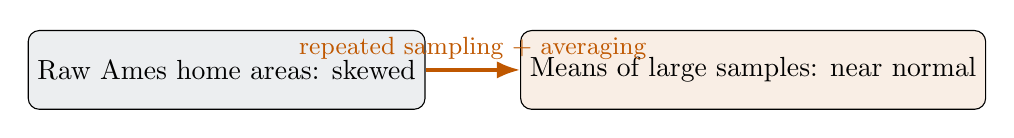
\begin{tikzpicture}[node distance=1.2cm]
\node[draw,rounded corners,fill=LBJnavy!8,minimum width=4cm,minimum height=1cm] (raw) {Raw Ames home areas: skewed};
\node[draw,rounded corners,fill=UTburnt!10,minimum width=4.3cm,minimum height=1cm,right=of raw] (means) {Means of large samples: near normal};
\draw[-{Latex},very thick,UTburnt] (raw)--node[above,font=\small]{repeated sampling + averaging}(means);
\end{tikzpicture}
\end{center}
\end{frame}

% 24
\begin{frame}{When can we use the CLT?}
Two ideas matter most.

\begin{enumerate}
  \item \textbf{Independence}
  \begin{itemize}
    \item Random sampling helps.
    \item If sampling without replacement, a common check is $n<10\%$ of the population.
  \end{itemize}

  \item \textbf{Population shape and sample size}
  \begin{itemize}
    \item Nearly normal population: small samples can work well.
    \item Moderate skew: larger $n$ improves the approximation.
    \item Strong skew or extreme outliers: we may need a much larger $n$.
  \end{itemize}
\end{enumerate}

\vfill
\alert{There is no universal magic cutoff where the CLT suddenly turns on.}
\end{frame}

% 25
\begin{frame}{Why ``$n=30$'' is only a rule of thumb}
\begin{columns}[T,onlytextwidth]
\column{0.47\textwidth}
\begin{block}{Mildly skewed population}
A sample size around 30 may already give a useful normal approximation for $\bar{x}$.
\end{block}
\column{0.47\textwidth}
\begin{block}{Very skewed population}
A sample size of 30 may still be too small if rare extreme values dominate the distribution.
\end{block}
\end{columns}

\vspace{0.9em}
The question is not simply ``Is $n\ge30$?''

\begin{center}
\Large It is: \alert{Is the approximation plausible for this data-generating process?}
\end{center}
\end{frame}

% 26
\begin{frame}{The key contrast from Lab 4}
Last Wednesday we asked about an \alert{individual} Ames home:
\[
P(X\ge 2000).
\]
Because home area is right-skewed, the normal model for individual homes is imperfect.

\vspace{0.8em}
Today we ask about the \alert{mean of 100 homes}:
\[
P(\bar{X}<1450).
\]
The CLT can make a normal approximation useful even though the original population is skewed.

\vfill
\alert{Individual observations and sample means have different distributions.}
\end{frame}

% 27
\begin{frame}{Our turn: probability for a sample mean}
For Ames home area,
\[
\mu=1499.69,\qquad \sigma=505.51,\qquad n=100.
\]

By the CLT,
\[
\begin{aligned}
\bar{X}&\approx N\!\left(\text{mean}=1499.69,\;\text{SD}=\frac{505.51}{\sqrt{100}}\right)\\
&=N(\text{mean}=1499.69,\;\text{SD}=50.55).
\end{aligned}
\]

What is $P(\bar{X}<1450)$?
\[
z=\frac{1450-1499.69}{50.55}\approx-0.98
\qquad\Longrightarrow\qquad
\boxed{P(\bar{X}<1450)\approx0.163}
\]
\end{frame}

% 28
\begin{frame}{What does 0.163 mean?}
\ourturn{Imagine repeatedly taking random samples of 100 Ames homes and calculating the mean living area each time.}

\vspace{0.8em}
A probability of about 0.163 means:

\begin{center}
\Large About \alert{16\%} of those samples would have\\
a sample mean below 1,450 square feet.
\end{center}

\vfill
It does \textbf{not} mean 16\% of individual homes are below 1,450 square feet.
\end{frame}

% 29
\begin{frame}[fragile]{The same calculation in R}
Once the sampling distribution is identified, R can calculate the tail area directly.

\begin{lstlisting}[language=R]
mu <- 1499.69
sigma <- 505.51
n <- 100

se <- sigma / sqrt(n)

pnorm(1450, mean = mu, sd = se)
# about 0.163
\end{lstlisting}

\vfill
The difficult part is usually not typing \texttt{pnorm()}. It is deciding \alert{which distribution} and \alert{which standard deviation} belong in the calculation.
\end{frame}

% 30
\begin{frame}{Transfer the idea to a policy setting}
Suppose a public benefits agency has processing times with
\[
\mu=42\text{ days},\qquad \sigma=18\text{ days}.
\]
A manager reviews a random sample of $n=81$ cases, so
\[
\SE(\bar{X})=\frac{18}{\sqrt{81}}=2\text{ days}.
\]
What is the probability the sample average exceeds 46 days?
\[
z=\frac{46-42}{2}=2
\qquad\Longrightarrow\qquad
\boxed{P(\bar{X}>46)\approx0.023}
\]

\begin{alertblock}{Interpretation}
A sample mean above 46 days would be relatively unusual if the long-run mean were really 42 days.
\end{alertblock}
\end{frame}

% 31
\begin{frame}{Your turn: change the sample size}
\yourturn{Keep $\mu=42$ and $\sigma=18$, but now sample only $n=36$ cases.
\begin{enumerate}
  \item What is the standard error?
  \item Is $P(\bar{X}>46)$ larger or smaller than it was for $n=81$?
  \item Why?
\end{enumerate}}

\[
\SE=\frac{18}{6}=3,
\qquad z=\frac{46-42}{3}=1.33,
\qquad P(\bar{X}>46)\approx0.092.
\]

\begin{alertblock}{Why did the probability grow?}
Smaller samples produce more variable means, so an average above 46 days is less unusual.
\end{alertblock}
\end{frame}

% 32
\begin{frame}{Why this matters for inference}
A point estimate alone does not tell us how precise it is.

\begin{center}
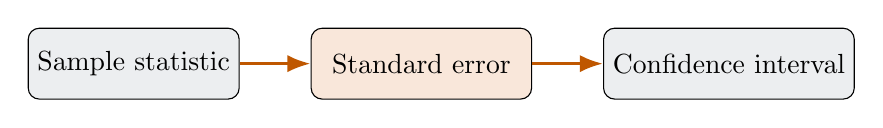
\begin{tikzpicture}[node distance=0.9cm]
\node[draw,rounded corners,fill=LBJnavy!8,minimum width=2.6cm,minimum height=0.9cm] (stat) {Sample statistic};
\node[draw,rounded corners,fill=softorange,minimum width=2.8cm,minimum height=0.9cm,right=of stat] (se) {Standard error};
\node[draw,rounded corners,fill=LBJnavy!8,minimum width=3.1cm,minimum height=0.9cm,right=of se] (ci) {Confidence interval};
\draw[-{Latex},very thick,UTburnt] (stat)--(se);
\draw[-{Latex},very thick,UTburnt] (se)--(ci);
\end{tikzpicture}
\end{center}

\vspace{1em}
A rough 95\% pattern for a normal sampling distribution is
\[
\text{estimate}\pm 2\times\SE.
\]

\vfill
Next: turn this logic into formal confidence intervals.
\end{frame}

% 33
\begin{frame}{Four traps to avoid}
\begin{enumerate}
  \item \textbf{Confusing SD with SE.} One describes observations; the other describes estimates.
  \item \textbf{Confusing the population distribution with the sampling distribution.}
  \item \textbf{Thinking larger $n$ changes the population mean.} It changes precision, not the target.
  \item \textbf{Treating $n=30$ as a law.} Normal approximation depends on shape and outliers too.
\end{enumerate}
\end{frame}

% 34
\begin{frame}{Today in four equations}
\begin{align*}
\text{Point estimate:}\qquad & \bar{x} \\[0.4em]
\text{Sampling-distribution center:}\qquad & E(\bar{X})=\mu \\[0.4em]
\text{Standard error:}\qquad & \SE(\bar{X})=\frac{\sigma}{\sqrt{n}} \\[0.4em]
\text{CLT:}\qquad & \bar{X}\approx N\!\left(\text{mean}=\mu,\;\text{SD}=\frac{\sigma}{\sqrt{n}}\right)
\end{align*}
\end{frame}

% 35
\begin{frame}[standout]
\Large Samples vary.\\[0.5em]
\Large Their variation is predictable.\\[0.7em]
\normalsize That predictability is what makes statistical inference possible.
\end{frame}

\end{document}
